\section{Discriminant Variables}\label{sec-vh-disc}
The analysis leverages a varied set of reconstructed kinematic variables in the fit to constrain the different processes and control mismodelling effects. Figure \ref{fig:variablesControlReg} displays the chosen variable used for each region in the fit in the resolved regime. The reconstructed Higgs mass offers some separation power to distinguish the signals from their major backgrounds, hence some control regions such as the top $BT$ \glspl{cr} and CRHighs are based on the relevant distributions $m_{bb}$, $m_{cc}$, or $m_J$, depending on the targeted decay and the regime. Some control regions passed to the fit are modelled with the $p_T^V$ distribution, such as the CRHighs in the 2L-channel $NT$ and $BB$ tagged-regions and the $V+l$ \gls{cr} ($LN$-tag). Directly fitting this distribution helps constrain an observed Monte Carlo mismodelling in the \ptv\ distributions of the \textsc{Sherpa} 2.2.11 $V+$jets samples, as detailed in Section \ref{sec-mod}. To optimise the signal and background separation in the statistical analysis, dedicated \glsreset{bdt}\glspl{bdt}, also called \glsreset{mva}\glspl{mva}, are trained for the signal regions of the combined analysis with the \textsc{TMVA} \textsc{Root} software \cite{Therhaag:2011jh}. Simple one-dimensional discriminants are built from the outputs of fine-tuned \glspl{bdt} trained on specific sets of event-level input variables, as described in detail in this section.

\subsection{Multivariate Analysis}
Three sets of \glspl{mva} discriminants are trained for the analysis: \textit{\gls{bdt}} discriminants for the signal region modelling, a specific set \textit{mvaCRLow} for the CRLow distribution in the resolved \vhb, and a set of \glspl{bdt} for the diboson cross-check analysis. For the last one, the signal is set to the diboson process decaying into the expected pair of jets $VZ(\rightarrow b\bar{b})$ or $VZ(\rightarrow c\bar{c})$, and the non-diboson processes as well as the $VH$ processes are considered as backgrounds. All multivariate discriminants predict a continuous score in the range $[-1, 1]$, with higher values indicative of a signal-like nature and lower values background-like. The wide adoption of \gls{bdt}-discriminants in all the regimes of the analysis marks a significant improvement over the standalone \vhc\ and boosted \vhb\ analyses, generalising the successful approach first introduced in the resolved \vhb\ \cite{ATLAS:2020fcp}.\\

\begin{figure}[h!]
  \center
  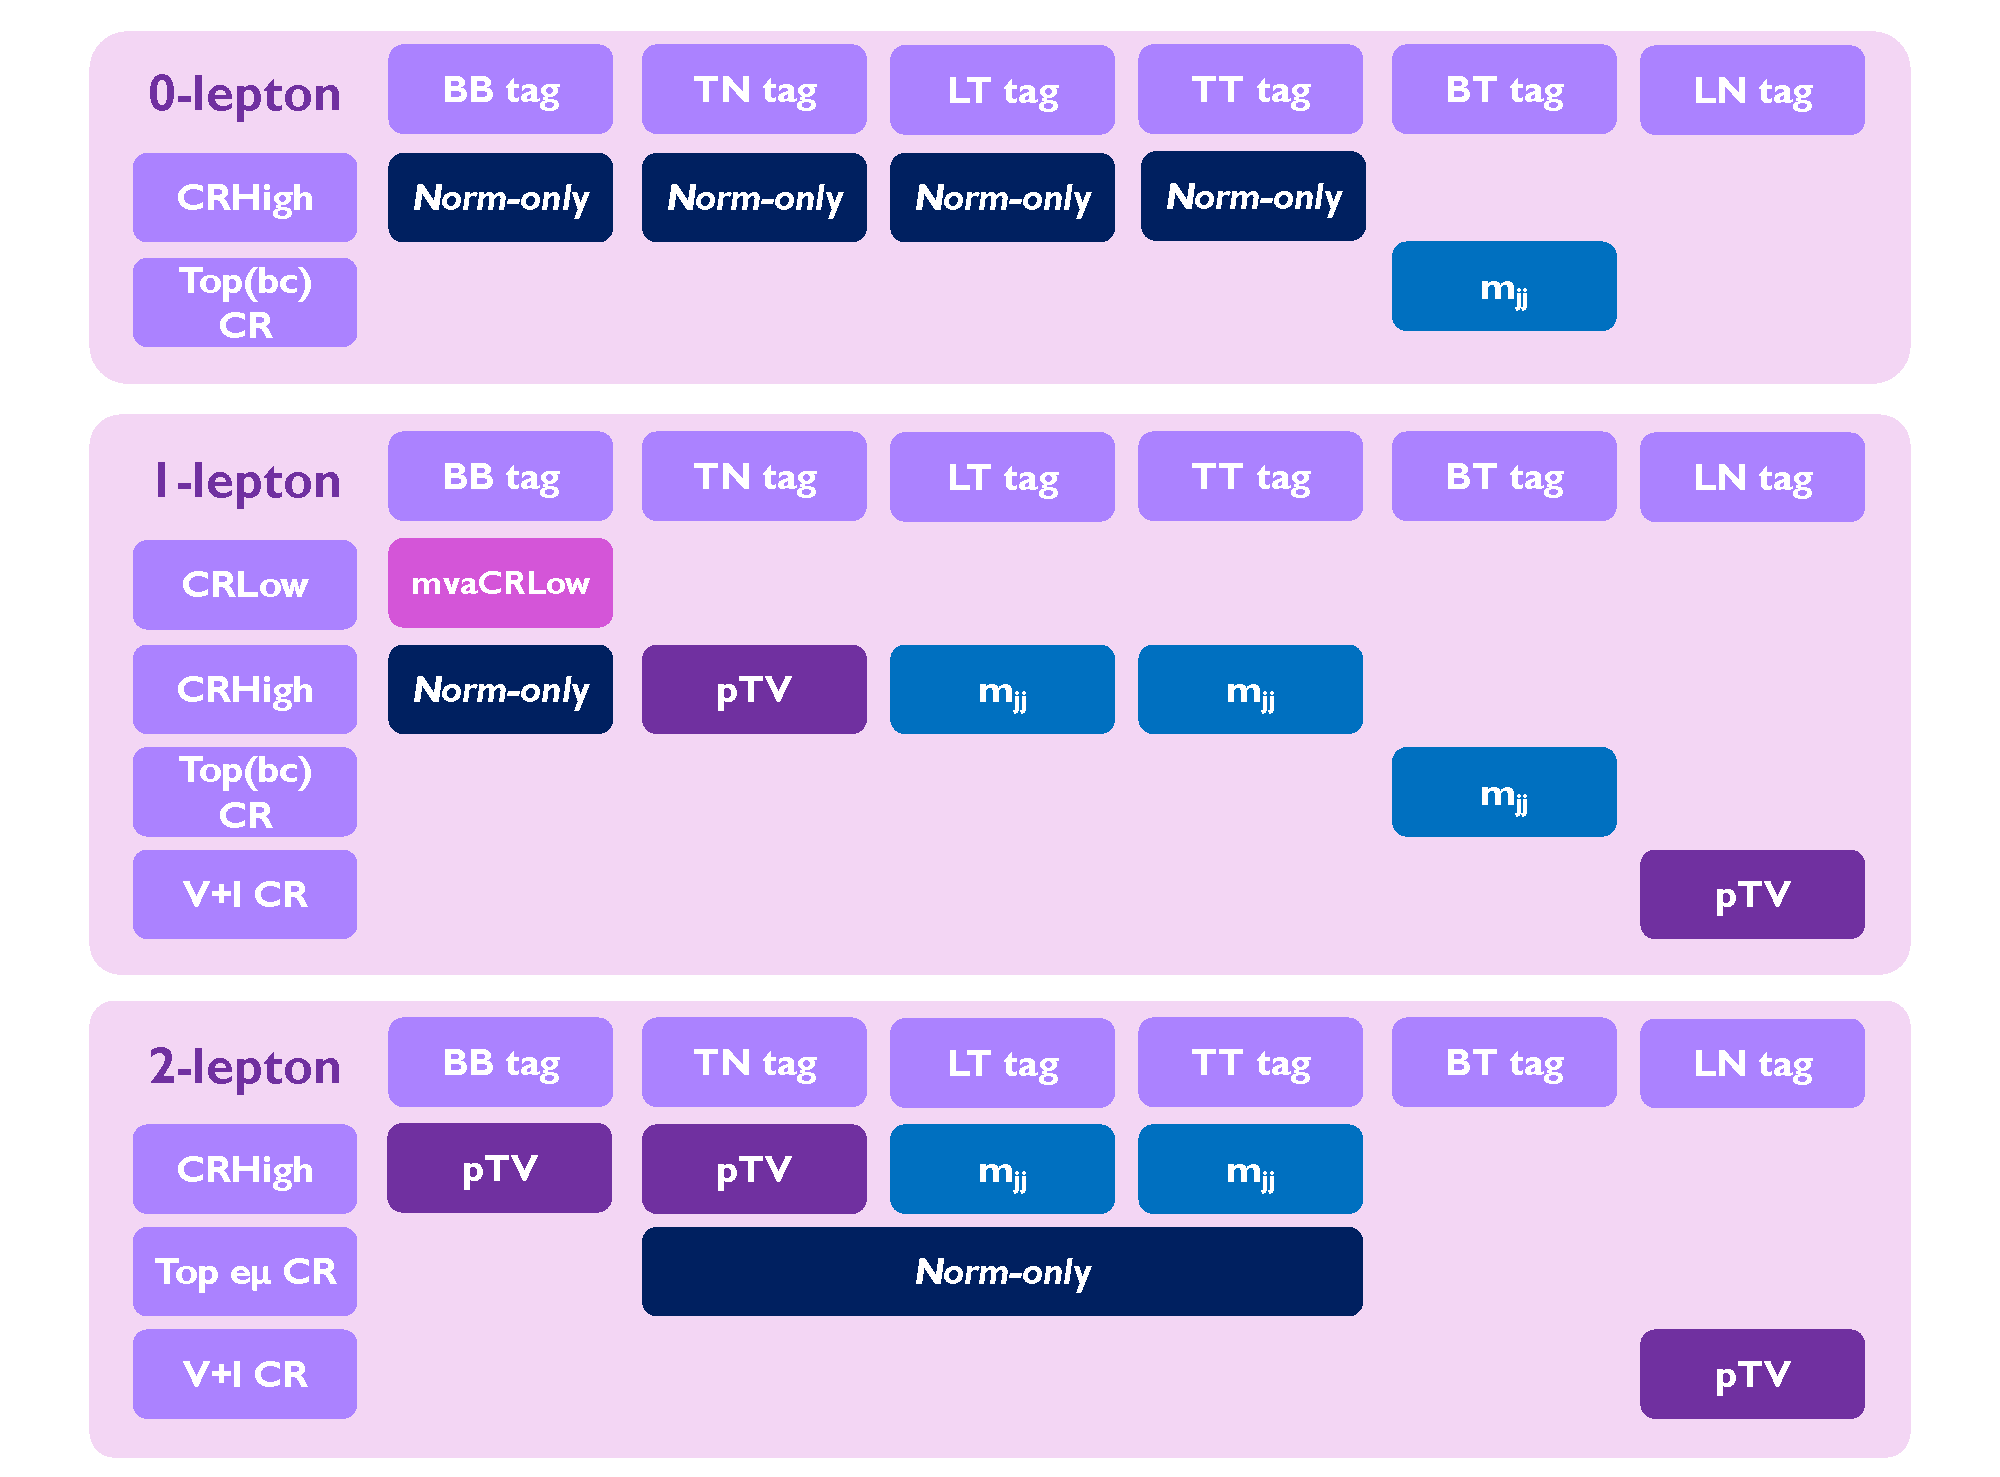
\includegraphics[width=0.98\textwidth]{Images/VH/Discriminants/Variables.pdf}
  \caption{Illustration of the discriminant variables used per control regions of the resolved regime in the statistical analysis. \textit{Norm-only} indicates a region included to extract a global normalisation, hence not binned by a variable.}
  \label{fig:variablesControlReg}
\end{figure}

Before training, the object and event selections of Section \ref{sec-selectionandcat} and the jet energy corrections of Section \ref{sec-vh-jetcor} are applied. To limit the number of training runs and the risk of overtraining from the low statistics of some kinematic regions, the \glspl{bdt} are trained on inclusive regions combining the \glspl{sr} and the $\Delta R$-based \glspl{cr}. The \glspl{bdt} are trained to discriminate the respective signal of the different targeted decays\footnote{The \vhb\ samples for the $BB$-tagged events and \vhc\ samples for the $c$-tagged events.} from background samples, including $V+$jets, \ttb, single-top, and diboson. \glspl{bdt} are specifically trained in the following categories, covering the fine analysis categorisation to guarantee sufficient statistics and avoid overtraining:
\begin{itemize}[leftmargin=*]
  \item \textbf{Resolved \boldvhbc:} \glspl{bdt} are trained separately for the $BB$tagged, 2 $c$-tagged, and 1 $c$-tagged events. Individual trainings are run for each lepton channel and for the following jet multiplicities and \ptv\ bins.
  \begin{itemize}
      \item \textbf{0L}: \glspl{bdt} are trained for the 2-, 3-, and 4-jet categories, each in an inclusive \ptv\ $\geq 150$ GeV region.
      \item \textbf{1L}: \glspl{bdt} are trained for the 2- and 3-jet categories, in the \ptv\ $\in [75, 150]$ GeV and \ptv\ $\geq 150$ GeV \ptv\ regions.
      \item \textbf{2L}: \glspl{bdt} are trained for the 2- and $\geq$3-jet categories, in the \ptv\ $\in [75, 150]$ GeV and \ptv\ $\geq 150$ GeV \ptv\ regions.
  \end{itemize}
  The low \ptv\ bin is separated from the higher \ptv\ $>$ 150 GeV due to its large statistics and different background compositions.
  \item \textbf{Boosted \boldvhbc:} a \gls{bdt} is trained per lepton channel, each in a single inclusive bin of \ptv\ $>400$ GeV.
\end{itemize}

For training, the full \gls{mc} samples statistics is leveraged thanks to the so-called \textit{GNN truth tagging} technique. Instead of filtering down the simulated samples by cutting away events failing to pass the flavour tagging requirements, as is done by the standard selection called \textit{direct tagging}, this technique applies a weight per event representing its probability of passing the tagging selection. The result is a weighted distribution possessing the statistical precision of the full \gls{mc} samples but distributed as the direct tagging scheme. The truth tagging weights are predicted by dedicated graph neural networks using event-level information, as detailed in Appendix \ref{app-truth-tagging}. The truth tagging procedure is applied separately to $BB$, $TT$, $TL$, and $NT$ events. \\

Each \gls{bdt} is trained with a specific set of features depending on the lepton channel, as listed in Table \ref{tbl:MVAVars} and detailed in Appendix \ref{ap-MVA}. Features with long tails are clipped to contain 99\% of the centred distributions. The chosen sets of features are the result of hyperparameter optimisation studies, with other variables tested but eventually not included due to their negligible impact on the performance. The architecture of the different \glspl{bdt} is also optimised, with the gradient boosting technique of Section \ref{sec-gradient-boost} deployed in the resolved regime to improve performance and capture effects outside the bulk of the distributions. In the boosted regime, due to the lower statistics available and large tails in the distributions, the AdaBoost method introduced in Section \ref{sub-adaboosted} is adopted to help stabilise the training \cite{Adaboost}. Tables \ref{tbl:MVAHyperparams} and \ref{tbl:MVAHyperparams-VHcc} list the architectures used for the \vhb\ and \vhc\ \glspl{bdt}, respectively, with the main and diboson \glspl{bdt} sharing the same hyperparameters. For \vhc, the hyperparameters are further tuned to avoid overtraining from the smaller available statistics in the 2L channel and the diboson cross-check. \\

Trainings are performed with the $k$-fold method, setting $k = 2$, to use the full statistics while assessing the overtraining risk. Each \gls{bdt} is therefore trained twice, once on odd events and once on even events. The performance is assessed on the held-out fold and the final discriminant is the combination of the odd- and even-trained \glspl{bdt}. Additional overtraining checks are performed on each fold comparing the trained distribution to a test distribution obtained by applying the \gls{bdt} on the held-out fold, as presented in Figure~\ref{fig:overtrainingCheck}. The good agreement between the training and test \gls{bdt} distributions indicates no overtraining occurred. The \glspl{bdt} deliver a good discrimination performance, with a typical \gls{auc} of the \gls{roc} of $\sim 0.9$ and a large increase on the expected statistical significance of the analysis compared to using the Higgs candidate mass as discriminating variable. \\

\newpage
\vspace*{\fill}
\begin{table}[!htbp]
    \hspace{-1cm}
    %\renewcommand*{\arraystretch}{1.3}
    \newcommand\textunderset[2]{\ensuremath{\underset{\textrm{#1}}{\textrm{#2}}}}
      %\setlength\aboverulesep{0pt}
      %\setlength\belowrulesep{0pt}
      % resize a bit the table 
      %\resizebox{1\textwidth}{!}{ %
      \begin{tabular}{c|ccc|ccc|M{6cm}}
        %\multicolumn{1}{c}{} & \multicolumn{3}{c}{\textunderset{Resolved}{\vhbc}} & \multicolumn{3}{c}{\textunderset{Boosted}{\vhb}} & \multicolumn{1}{c}{}
        \multicolumn{1}{c}{} & \multicolumn{3}{c|}{\vhbc} & \multicolumn{3}{c}{\vhb} & \multicolumn{1}{c}{}\\
        \multicolumn{1}{c}{} & \multicolumn{3}{c|}{Resolved} & \multicolumn{3}{c}{Boosted} & \multicolumn{1}{c}{}
        \\ \hline \hline
        Variable & 0L & 1L & 2L & 0L & 1L & 2L 
        \\ \hline
        $m_{j_1j_2}$ or $m_J$
            & \checkmark & \checkmark & \checkmark 
            & \checkmark & \checkmark  & \checkmark 
            & Mass of Higgs candidate
        \\ \hline
        $m_{{j_1 j_2 j_3}}$ 
            & \checkmark & \checkmark & \checkmark 
            & & &
            & Mass of Higgs candidates and leading additional jets
        \\ \hline
        $p_T^{j_1}$
            & \checkmark & \checkmark & \checkmark 
            & \checkmark & \checkmark & \checkmark 
            & Leading Higgs candidate $p_T$
        \\ \hline
        $p_T^{j_2}$
            & \checkmark & \checkmark & \checkmark 
            & \checkmark & \checkmark & \checkmark 
            & Subleading Higgs candidate $p_T$
        \\ \hline
        $p_T^{j_3}$ 
            & & & 
            & \checkmark & \checkmark & \checkmark 
            & Leading non-Higgs candidate $p_T$
        \\ \hline
        $\sum\limits_{i\neq 1, 2}p_T^{j_i}$ 
            & \checkmark & \checkmark & \checkmark 
            & & & 
            & Sum of non-Higgs jet $p_T$
        \\ \hline
        $\Delta R(\boldsymbol{j_1}, \boldsymbol{j_2})$
            & \checkmark & \checkmark & \checkmark 
            & \checkmark & \checkmark & \checkmark 
            & Angular separation of Higgs candidates
        \\ \hline
        $\mathrm{bin}_{\mathrm{DL1r}}(j_1)$ 
            & \checkmark & \checkmark & \checkmark
            & \checkmark & \checkmark & \checkmark 
            & Tag bin of $j_1$
        \\ \hline
        $\mathrm{bin}_{\mathrm{DL1r}}(j_2)$ 
            & \checkmark & \checkmark & \checkmark
            & \checkmark & \checkmark & \checkmark 
            & Tag bin of $j_2$
        \\ \hline
        \ptv 
            & $\equiv E_T^{\textrm{miss}}$ & \checkmark  & \checkmark
            & $\equiv E_T^{\textrm{miss}}$ & \checkmark  & \checkmark
            & Vector boson $p_T$
        \\ \hline
        $E_T^{\textrm{miss}}$
            & \checkmark & \checkmark & 
            & \checkmark & \checkmark & 
            & Missing transverse energy
        \\ \hline
        $E_T^{\textrm{miss}}/\sqrt{S_T}$
            & & & \checkmark 
            & & & 
            & Ratio of \etm\ to sum of jets $p_T$
        \\ \hline
        $|\Delta y(\boldsymbol{V},\boldsymbol{H})|$
            & & \checkmark & \checkmark
            & & \checkmark & \checkmark
            & Rapidity between $V$ and $H$
        \\ \hline
        $|\Delta \phi(\boldsymbol{V},\boldsymbol{H})|$
            & \checkmark & \checkmark & \checkmark
            & \checkmark & \checkmark & \checkmark
            & Azimuthal angle between $V$ and $H$
        \\ \hline
        $|\Delta \eta(\boldsymbol{j_1},\boldsymbol{j_2})|$
            & \checkmark & & 
            & & & 
            & Pseudorapidity distance between Higgs candidates
        \\ \hline
        $\min\Delta R(j_i, j)_{i=1,2}$
            & \checkmark & \checkmark & 
            & & & 
            & Smallest angular distance between a Higgs and non-Higgs candidates
        \\ \hline
        $\mathrm{min}[\Delta\phi(\boldsymbol{\ell},\boldsymbol{j_1} \textrm{~or~} \boldsymbol{j_2})]$
            & & \checkmark  &
            & & & 
            & Smallest $\phi$ between the lepton and a Higgs candidate
        \\ \hline
        $m_{\textrm{eff}}$
            & \checkmark & & 
            & & &
            & Scalar sum of $p_T$ of all small-$R$ jet and \etm
        \\ \hline
        $m_T^W$
            & & \checkmark &
            & & &
            & Transverse mass of the $W$
        \\ \hline
        $m_{\textrm{top}}$
            & & \checkmark &
            & & &
            & Mass of reconstructed top-quark decaying semi-leptonically
        \\ \hline
        $m_{\ell\ell}$
            & & & \checkmark 
            & & & 
            & Mass of di-lepton system
        \\ \hline
        $\cos{\theta(\boldsymbol{\ell^-},\boldsymbol{Z})}$
            & & & \checkmark 
            & & & \checkmark 
            & $Z$ boson polarisation sensitive angle
        \\ \hline
        $(p_T^{\ell_1} - E_T^{\textrm{miss}})/p_T^W$
            & & &
            & & \checkmark & 
        \\ \hline
        $p_T^{\ell}$
            & & &
            & & \checkmark & 
            & \pt\ imbalance of the lepton and neutrino from $W$ 
        \\ \hline
        $N(\textrm{track-jets in }J)$
            & & & 
            & \checkmark & \checkmark & \checkmark
            & Number of track-jets associated to leading-$R$ jet
        \\ \hline
        $N(\textrm{add. small R-jets})$
            & & & 
            & \checkmark & \checkmark & \checkmark
            & Number of additional small-$R$ jets not matched
        \\ \hline
        Colour
            & & & 
            & \checkmark & \checkmark & \checkmark
            & Variable modelling colour-flow from \gls{qcd}
        \\ \hline \hline
      \end{tabular}
      %}
      \caption{%
        The variables used for the 0L, 1L, and 2L channels MVA's in the resolved and boosted regimes for the \vhbc\ combined analysis. The variables are further described in Appendix \ref{ap-MVA}.}%
      \label{tbl:MVAVars}
    \end{table}
  
\vspace*{\fill}
\newpage
\vspace*{\fill}
\begin{table}[!htbp]
  \renewcommand*{\arraystretch}{1.3}
  \newcommand\textunderset[2]{\ensuremath{\underset{\text{#1}}{\text{#2}}}}
  \centering
    % resize a bit the table 
    \resizebox{1\textwidth}{!}{%
    \begin{tabular}{c|ccc|ccc}
      \multicolumn{1}{c}{} & \multicolumn{3}{c|}{Resolved \vhb} &  \multicolumn{3}{c}{Boosted \vhb} 
      \\\hline \hline
      \textbf{Settings} & 0L & 1L & 2L & 0L & 1L & 2L
      \\\hline
      Boost type 
        & Gradient boost & Gradient boost & Gradient boost % VHbb Resolved 
        & Adaboost       & Adaboost       & Adaboost       % VHbb Boosted 
      \\\hline 
      Number of trees 
        & 200 & 600 & 200 % VHbb Resolved 
        & 800 & 800 & 400 % VHbb Boosted 
      \\\hline 
      Maximum depth
        & 3 & 4 & 4 % VHbb Resolved 
        & 3 & 3 & 3 % VHbb Boosted 
      \\\hline 
      Learning rate ($\beta$) 
        & 0.5 & 0.5 & 0.5% VHbb Resolved 
        & 0.5 & 0.35 & 0.3 % VHbb Boosted 
      \\\hline 
      Number of cuts
        & 100 & 100 & 100% VHbb Resolved 
        & 60  & 60  & 100 % VHbb Boosted 
      \\\hline 
      Minimum node size 
        & 5\% & 5\% & 5\% % VHbb Resolved 
        & 2\% & 2\% & 7\% % VHbb Boosted 
      \\ \hline \hline
    \end{tabular}}%
  \caption{%
    Hyperparameters of the BDTs in the 0L, 1L and 2L channels for the \vhb resolved and boosted. All models used the Gini index as separation method, without pruning.}%
  \label{tbl:MVAHyperparams}
\end{table}


% VHcc use different hyper parameters
\begin{table}[!htbp]
  \renewcommand*{\arraystretch}{1.3}
  \newcommand\textunderset[2]{\ensuremath{\underset{\text{#1}}{\text{#2}}}}
  \centering
    % resize a bit the table 
    %\resizebox{1\textwidth}{!}{%
    \begin{tabular}{c|cc|c}
      \multicolumn{1}{c}{} & \multicolumn{2}{c|}{\vhc} &  $VZ{\rightarrow c\bar{c}}$ signal
      \\\hline \hline
      \textbf{Settings} & 0L, 1L and most 2L regions & 2  3p-jet, low pTV & 0L, 1L and 2L
      \\\hline
      Boost type 
        & Gradient boost & Adaboost % VHcc
        & Adaboost                  % VZcc
      \\\hline 
      Number of trees 
        & 600 & 200 % VHcc
        & 200       % VZcc 
      \\\hline 
      Maximum depth
        & 4 & 4     % VHcc
        & 4         % VZcc
      \\\hline 
      Learning rate ($\beta$) 
        & 0.5 & 0.15 % VHcc
        & 0.15       % VZcc 
      \\\hline 
      Number of cuts
        & 100 & 100  % VHcc
        & 100        % VZcc
      \\\hline 
      Minimum node size 
        & 5\% & 5\%  % VHcc
        & 5\%        % VZcc
      \\ \hline \hline
    \end{tabular}
  %}
  \caption{%
    Hyperparameters of the BDTs in the 0L, 1L and 2L channels of \vhc. The 2L low pTV region mentioned is 75 GeV $<$ pTV $<$ 150 GeV. All models used the Gini index as separation method, without pruning.}%
  \label{tbl:MVAHyperparams-VHcc}
\end{table}


\begin{figure}[h!]
  \hspace{-0.3cm}
  \begin{subfigure}[b]{0.49\textwidth}
      \centering
    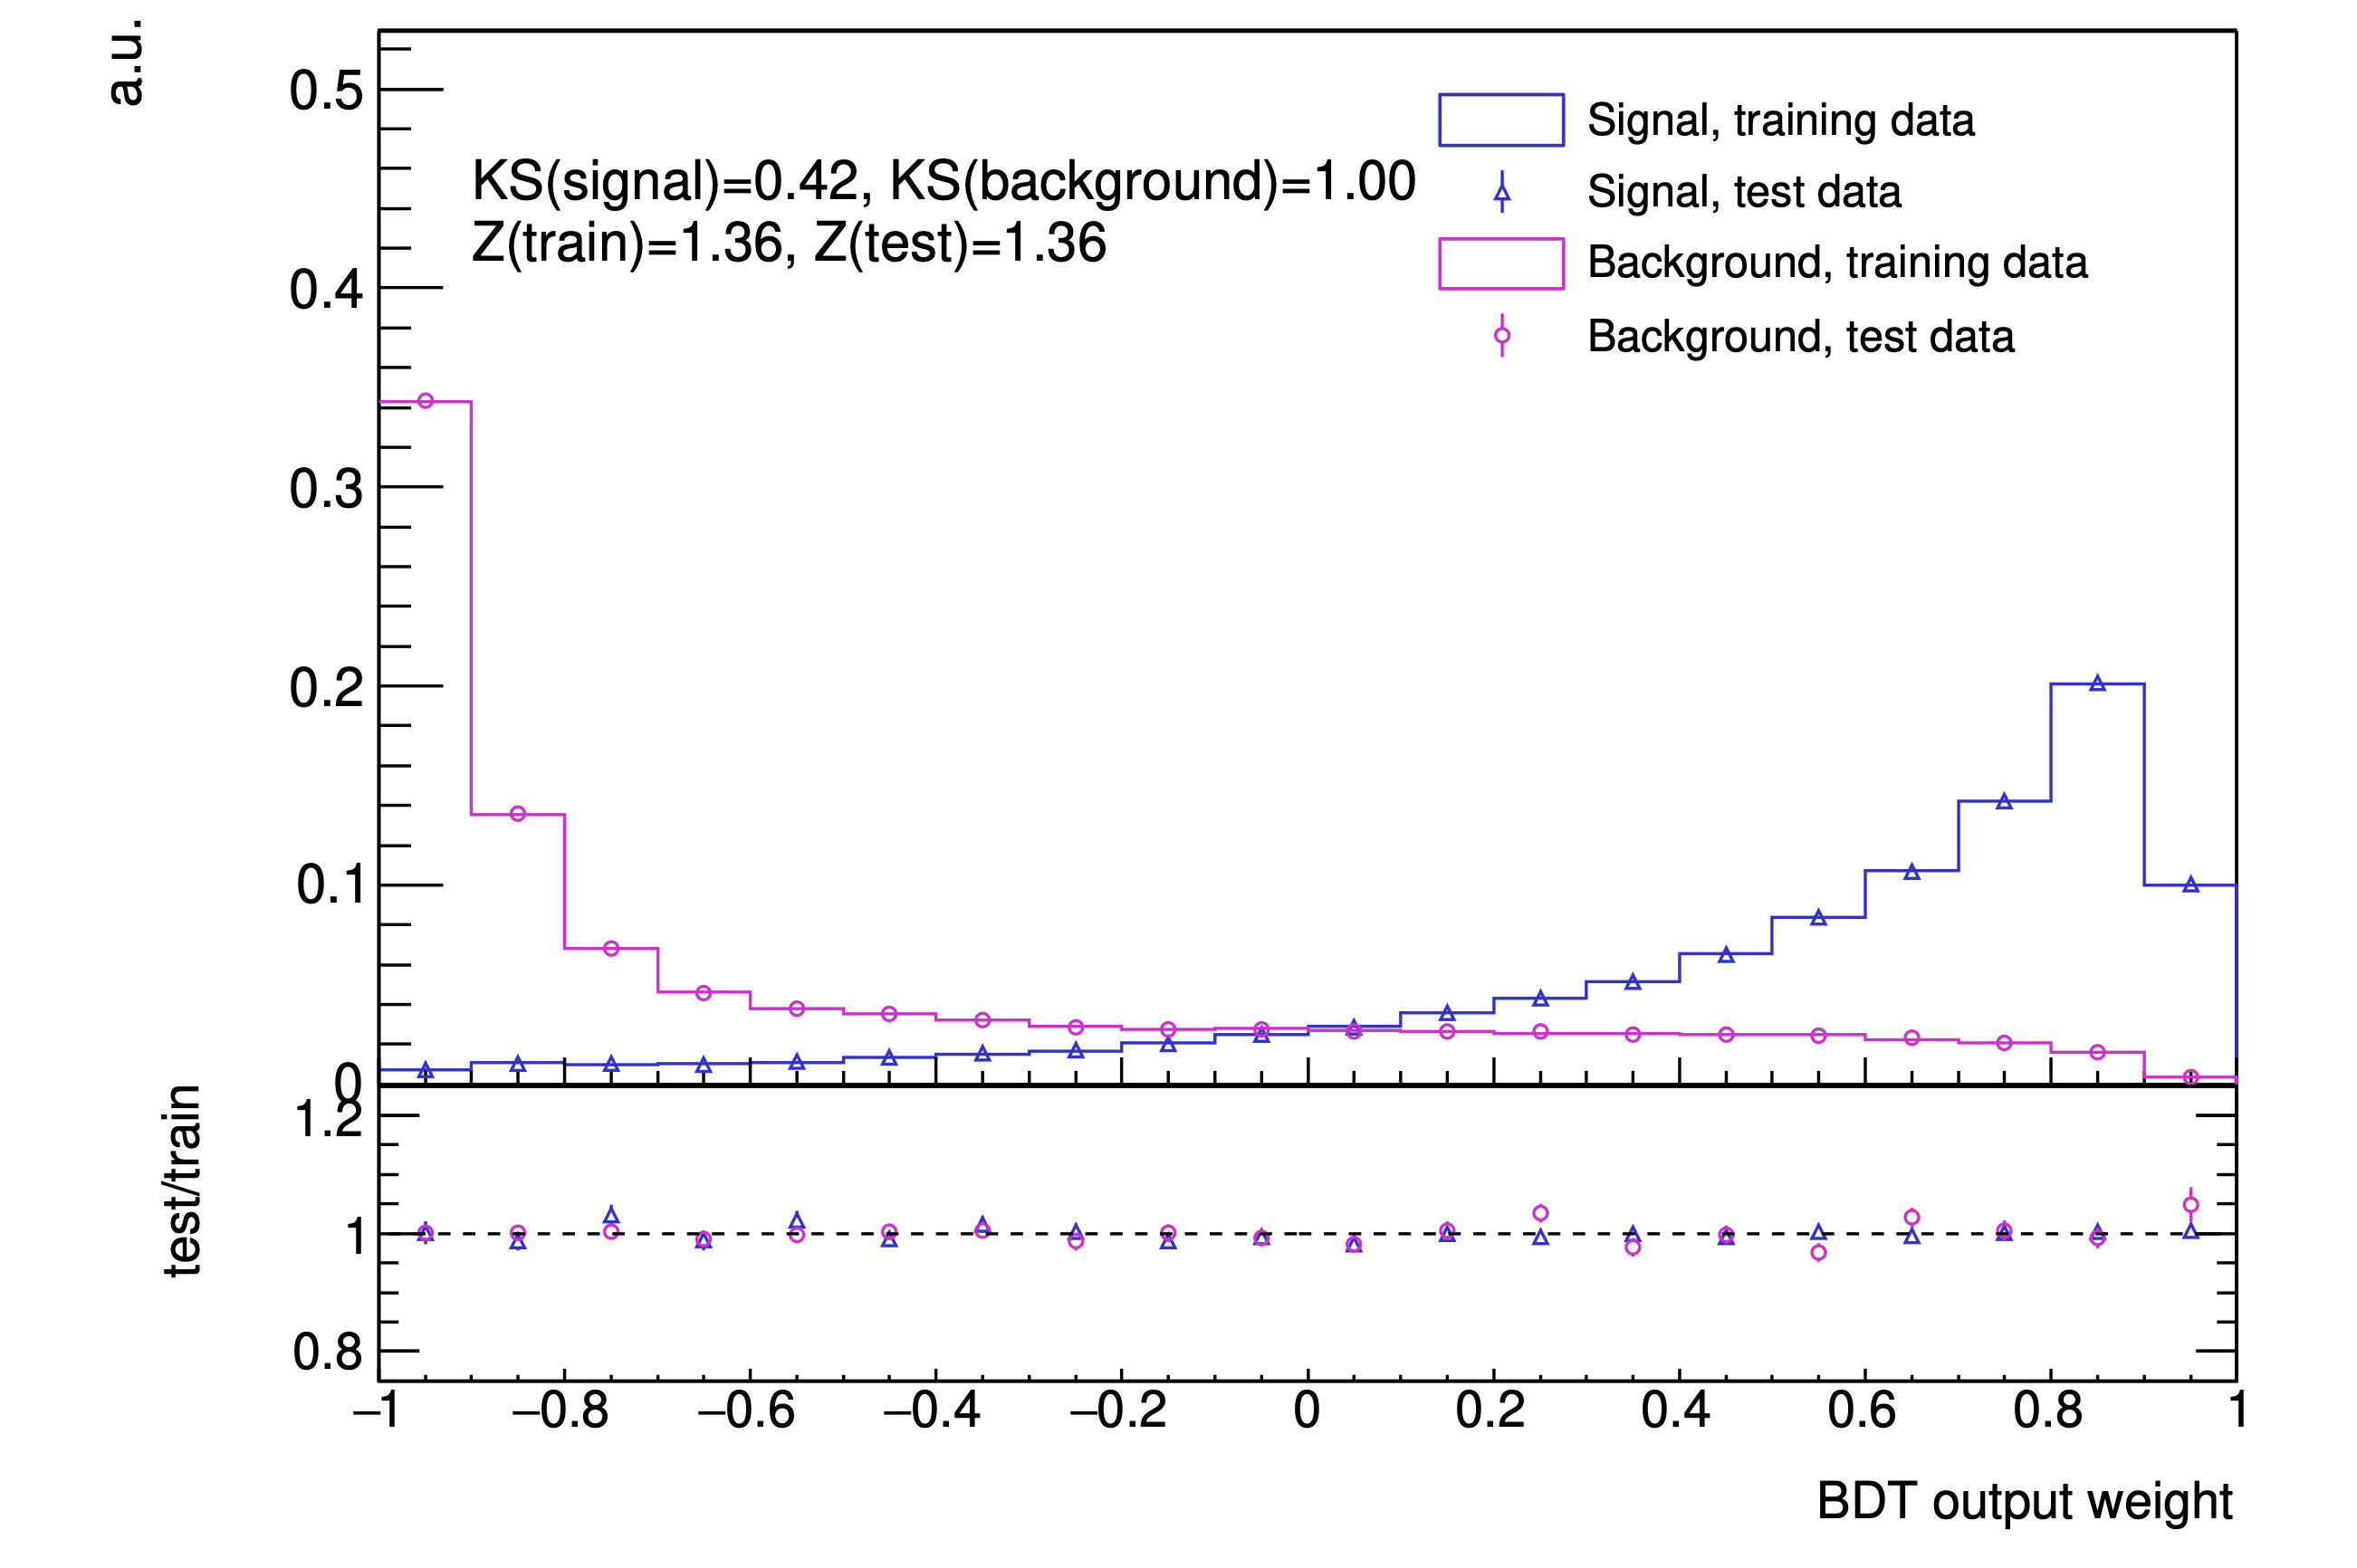
\includegraphics[width=\textwidth]{Images/VH/Discriminants/0Lbb.png}
  \caption{$BB$-tagged model, test AUC = 0.9.} 
  \end{subfigure}
  \begin{subfigure}[b]{0.49\textwidth}
      \centering
    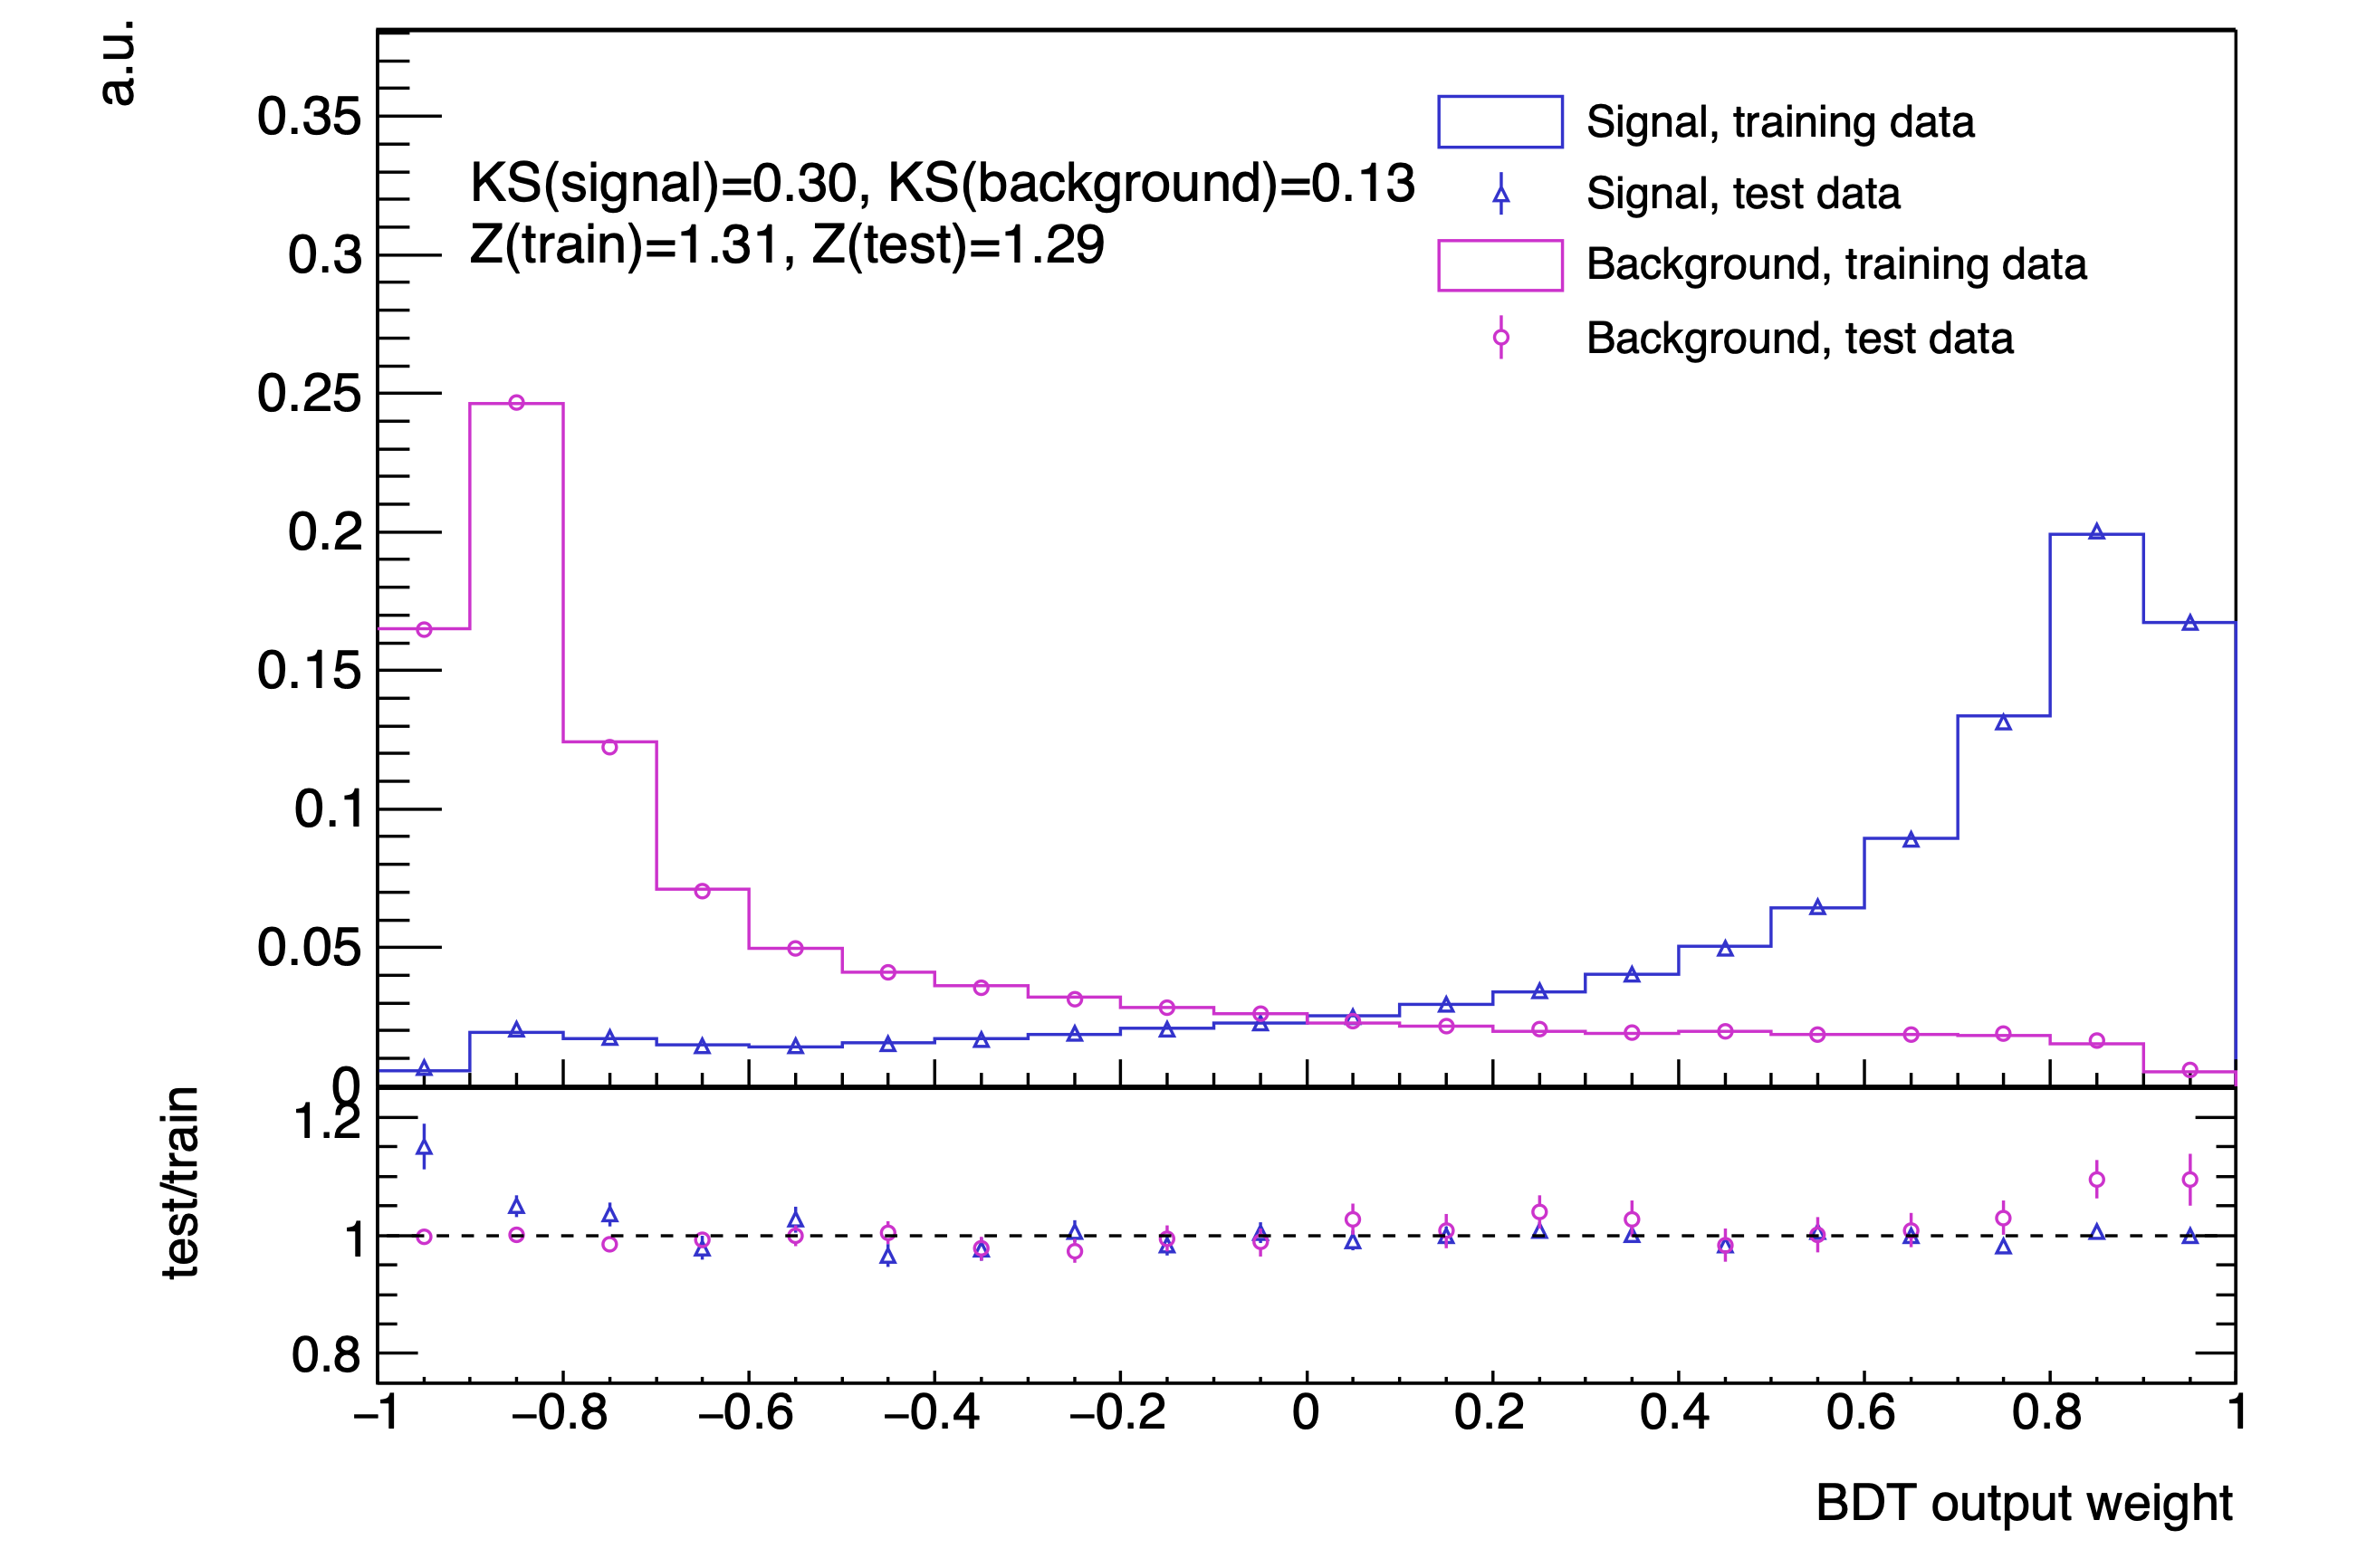
\includegraphics[width=\textwidth]{Images/VH/Discriminants/0Lcc.png}
    \caption{2 $c$-tagged model, test AUC = 0.898.}
  \end{subfigure}
  \caption{Overtraining checks for the BDTs trained for the resolved \vhb\ (left) and \vhc\ (right) in the 0L 2-jet region with \ptv\ $\geq$ 150 GeV. The binned histograms are the training data (blue) and background (purple) \gls{bdt} distributions, while the data points are the equivalent for the test sets. The bottom panels show the ratio of test/train.}
  \label{fig:overtrainingCheck}
\end{figure}
\vspace*{\fill}
\newpage

In addition to the signal and cross-checks \glspl{mva}, additional \glspl{mva} are trained for the \vhb\ resolved 1L channel in the \lowdr\ \gls{cr}. This region is dedicated to the $W+$jets process, with a rich contribution of the important $W+bb$ background. At low \ptv, there is unfortunately also a large contribution from \ttb, reducing the purity of the $W+bb$ in this \gls{cr}. To recover a higher sensitivity to the $W+$jets background, \glspl{mva} are specially trained to discriminate the $W+bb$ process from other backgrounds in the CRLow events. They are trained with 2-fold on truth tagged samples, separately for the \ptv\ $< 150$ GeV and \ptv\ $> 150$ GeV, in a single inclusive jet multiplicity bin combining the 2- and 3-jet categories. The typical \gls{auc} of these discriminants is $\sim0.84$, with no overtraining observed.

\subsection{Output Variable Transformation}
The \glspl{bdt} outputs from the previous section are finely-binned \gls{mva} variables maximising the separation of signals from backgrounds. To optimise the sensitivity of the statistical analysis, the \gls{mva} distributions are rebinned such that low \gls{bdt} scores are still indicative of a background-like event and larger values are signal-like. This rebinning is performed with attention given to the statistical uncertainty in each bin and the final sensitivity of the discriminant score. The analysis relies on the so-called \textit{Transformation D} algorithm., defining a per-bin score $Z$ as
\begin{equation}
    Z = z_s \frac{n_s}{N_s} + z_b \frac{n_b}{N_b},
\end{equation} 
where $N_s$ ($N_b$) is the total number of signal (background) events, $n_s$ ($n_b$) the number of signal (background) events in a specific bin, and $z_s$ and $z_b$ are tunable parameters indirectly controlling the number of signal and background bins desired in the region. For a given choice of $z_s$ and $z_b$, the algorithm starts from the initial binning of the \glspl{bdt} and successively recombines bins from the higher bin values (right) to the lower values (left) of the distribution. Successive bins of the original distribution are merged until the combined bin reaches a score $Z > 1$, thanks to increases in $n_s$ and $n_b$. Once a combined bin reaches the desired scores, it is removed from consideration and the algorithm starts again from the highest bin not yet recombined.\\
\begin{table}[h!]
  \resizebox{\textwidth}{!}{
  \begin{tabular}{c|c|c|c|c|c}
    \hline\hline
    %& $75 < p_T^V <150~\text{GeV}$ & $150 < p_T^V <250~\text{GeV}$ & $250 < p_T^V <400~\text{GeV}$ & $400 < p_T^V <600~\text{GeV}$ & \multicolumn{1}{c}{$p_T^V >600~\text{GeV}$}\\ \hline
    \ptv\ & $[75, 150]$ GeV & $[150, 250]$ GeV & $[250, 600]$ GeV & \multicolumn{1}{c}{$p_T^V >600~\text{GeV}$}\\ \hline
    \vhb\ & \multicolumn{2}{c|}{$z_s = 10,\ z_b = 5$} & $z_s=5,\ z_b=3$ & \multicolumn{1}{c}{$\begin{cases} \text{0L/1L: } z_s = 3, z_b = 2 \\ \text{2L: }z_s = 2, z_b = 2\end{cases}$}\\\hline
   \vhc\ & 
   $\begin{cases} % 75-150
      \text{$TT$: } z_s = 5, z_b = 3 \\
      \text{Else: } z_s = 10,\ z_b = 5
    \end{cases}$ & 
    
    $\begin{cases} % 150L250
      \text{0L/1L} & \begin{cases} 
                            \text{$TT$: } z_s = 5, z_b = 3 \\
                            \text{Else: } z_s = 10,\ z_b = 5
                          \end{cases}\\
      \text{2L} & \begin{cases}
                          \text{$TT$: } z_s = 2,\ z_b = 2\\
                          \text{$LT$/$XT$: } z_s = 5,\ z_b = 5\\
                          \text{Else: } z_s = 10,\ z_b = 5
                        \end{cases}
    \end{cases}$
      & \multicolumn{2}{l}{
        $\begin{cases} \text{$TT$: } z_s = 2, z_b = 2 \\ %250L400
                        \text{$LT$/$XT$: } z_s = 5,\ z_b = 3 \\
                        \text{Else: } z_s = 10,\ z_b = 5
        \end{cases}$
      }
    \\\hline \hline
  \end{tabular}
  }
  \caption{The optimised tune of the $z_s$ and $z_b$ parameter to rebin the MVAs with the \textit{Transformation D} algorithm in different regimes of the combined analysis.}
  \label{tab:trafoDParams}
\end{table}

The $z_s$ and $z_b$ parameters are tuned for each analysis regime and lepton channel, giving signal regions with a final number of \gls{bdt} bins varying from 4 to 15, as displayed in the postfit plots of Appendix \ref{appsec-vh-analRegPosfit}. An additional protection is added to avoid bins with too low data or \gls{mc} statistics, requiring at least 3 signal + background events per bin after transformation. The specific tunes for the different regimes of the combined analysis are presented in Table~\ref{tab:trafoDParams}.
\newpage